\documentclass[11pt]{scrartcl}
\usepackage{ngerman}	%Benutzung deutscher Umlaute
\usepackage{pgf}		%Zum Einbinden von JPEG
\usepackage{amsmath}	%Einrücken von Gleichungen z.B. durch gather
\usepackage{mdframed}	%Ermöglicht farbige Rahmen
\usepackage{amssymb}	%Korrekte Darstellung von phi

\author{Alex Jäger}
\title{Formelsammlung Hochfrequenztechnik}
\date{\today}

\def\Uc{\underline{\hat U}}
\def\Ic{\underline{\hat I}}

\definecolor{sand}{RGB}{240, 230, 140}	%Farbe für Formelkästen
 

\begin{document}

\maketitle
\newpage
\section{Grundlegende Formeln}
\begin{align*}
	\lambda_0 & \hat{=}\text{ Wellenlänge im Vakuum} \\
	v_{ph} & \hat{=}\text{ Phasengeschwindigkeit} \\
	T&=\frac{1}{f} \\
	\lambda _0&=\frac{c_0}{f} \\
	\lambda&=\frac{\lambda_0}{\sqrt{\epsilon_R}} \\
	v_{ph}&=\frac{c_0}{\sqrt{\epsilon_R}}
\end{align*}
\begin{center}
	Zusammenhang komplexer Zeiger und Zeitfunktion
\end{center}
\begin{align*}
	u(t) & \hat{=} \text{ Zeitfunktion} \\
	\Uc & \hat{=} \text{ Komplexer Amplitudenzeiger} \\
	\Uc(x) & \hat{=} \text{ Komplexer Amplitudenzeiger an der Stelle x} \\
	\Uc_0 & \hat{=} \text{ Komplexer Amplitudenzeiger bei x=0} \\
	u(t)&=Re\{\Uc e^{j\omega t}\} \\
	\Uc &=\hat U*e^{j\varphi} \\
	\Uc(x)&=\Uc_0*e^{\gamma x}
\end{align*}

\section{Leitungstheorie}
\subsection{Leitungsmodell}
\begin{center}
	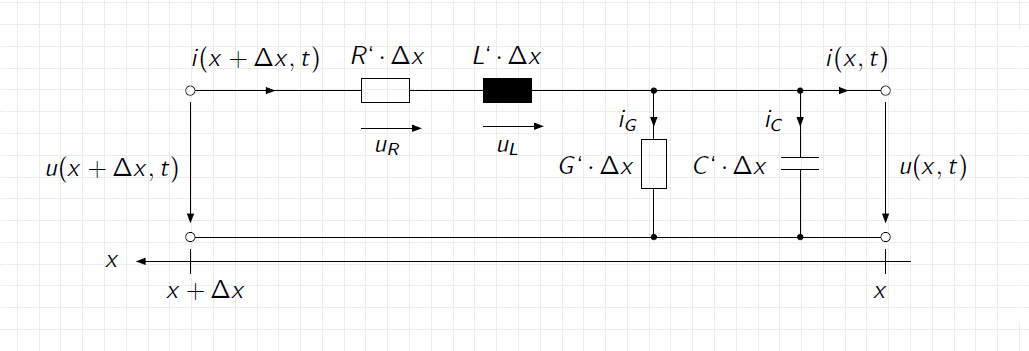
\includegraphics[width=\textwidth]{Grafiken/01_Leitungsmodell.png}
\end{center}
Kirchhoff'sche Regel führt z.B. zu
\begin{gather*}
	u_R+u_L+u(x,t)-u(x+\Delta x,t)=0 \\	
	R'*\Delta x*i(x+\Delta x,t)+L'*\Delta x*\frac{\partial i(x+\Delta x,t)}{\partial t}+u(x,t)-u(x+\Delta x,t)=0
\end{gather*}
oder
\begin{gather*}
	i(x+\Delta x,t)-i_g-i_c-i(x,t)=0 \\
	i(x+\Delta x,t)-G'*\Delta x*u(x,t)-C'*\Delta x*\frac{\partial u(x,t)}{\partial t}-i(x,t)=0
\end{gather*}
	\subsection{Telegraphengleichungen}
	\begin{eqnarray*}
		\frac{\partial u(x,t)}{\partial x}=R'*i(x,t)+L'*\frac{\partial i(x,t)}{\partial t}\\
		\frac{\partial i(x,t)}{\partial x}=G'*u(x,t)+C'*\frac{\partial u(x,t)}{\partial t}
	\end{eqnarray*}
	Daraus folgt
	\begin{eqnarray*}
		\frac{\partial ^2u(x,t)}{\partial x^2}=L'C'\frac{\partial ^2u(x,t)}{\partial t^2}+(R'C'+L'G')\frac{\partial u(x,t)}{\partial t}+R'G'*u(x,t)
	\end{eqnarray*}
	\subsubsection{Telegraphengleichungen im Komplexen}
	\begin{align}
		\frac{\partial \Uc(x)}{\partial x}&=(R'+j\omega L')*\Ic(x) \\
		\frac{\partial \Ic(x)}{\partial x}&=(G'+j\omega C')*\Uc(x) \\
		\frac{\partial ^2\Uc(x)}{\partial x^2}&=L'C'(j\omega)^2*\Uc(x)+(R'C'+L'G')j\omega*\Uc(x)+R'G'\Uc(x)	
	\end{align}
Durch Einsetzen von $\Uc(x)=\Uc_0e^{\gamma x}$ folgt
\begin{eqnarray*}
	\gamma_{1,2}=\pm \sqrt{(R'+j\omega L')+(G'+j\omega C')} \\
	\gamma_{1,2}=\pm (\alpha+j\beta) \text{ mit } \beta=\frac{2\pi}{\lambda}
\end{eqnarray*} 

\subsection{Spannungszeiger an der Position x als Summe fort- und rücklaufender Welle}
\begin{eqnarray*}
	\Uc(x)=\Uc_F(x)+\Uc_B(x) \\
	\Uc(x)=\Uc_{0F} e^{\gamma x} + \Uc_{0B} e^{-\gamma x}
\end{eqnarray*}
Hinweis: Der Stromzeiger ergibt sich als Differenz der anderen Stromzeiger.
\begin{equation*}
	\Ic(x)=\Ic_{0F} e^{\gamma x} - \Ic_{0B} e^{-\gamma x}
\end{equation*}
\subsection{Charakteristische Impedanz einer Leitung}
\begin{mdframed}[backgroundcolor = sand]
	\begin{equation}
		\underline{Z}_0 = \frac{R'+j\omega L'}{\gamma} = \sqrt{\frac{R'+j\omega L'}{G' + j \omega C'}}
	\end{equation}
\end{mdframed}
\begin{equation}
\Ic(x) = \frac{1}{\underline{Z}_0} * (\Uc_{0F}  e^{\gamma x} - \Uc_{0B}  e^{-\gamma x})
\end{equation}
	

\subsection{Reflexionskoeffizient verlustfreier Leitungen}
Trifft eine Leitung der charakteristische Impedanz $Z_0$ auf einen Widerstand der Impedanz $\underline{Z}_2$ (Hinweis: $Z_0 \in \mathbb{R}$, weil die Leitung verlustfrei ist), so ergibt sich eine Reflexion mit dem Faktor
\begin{equation*}
	\underline{r} = \frac{\Uc_B}{\Uc_F}
\end{equation*}
An der Position x=0 gilt
\begin{mdframed}[backgroundcolor = sand]
	\begin{equation*}
		\underline{r}(x=0) = \frac{\underline{Z}_2-Z_0}{\underline{Z}_2+Z_0} 
	\end{equation*}
\end{mdframed}
\subsection{Gesamtimpedanz von Leitung und Widerstand}
\begin{center}
	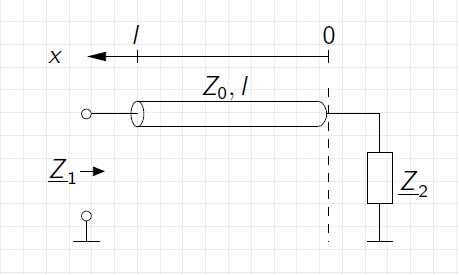
\includegraphics[width=0.3\textwidth]{Grafiken/02_Leitungsimpedanz.png}
\end{center}
\begin{equation*}
	\underline{Z}_1 = Z_0*\frac{\underline{Z}_2+jZ_0tan(\beta l)}{Z_0+j\underline{Z}_2tan(\beta l)}
\end{equation*}
Daraus folgt für $\underline{Z}_2 = 0$
\begin{equation*}
	\underline{Z}_1 = jZ_0tan(\beta l)
\end{equation*}
und für $\underline{Z}_2\rightarrow\infty$
\begin{equation*}
	\underline{Z}_1 = -jZ_0\frac{1}{tan(\beta l)}
\end{equation*}
\subsection{Leistung am Widerstand}
Falls $\underline{r} = 0$ gilt
\begin{equation*}
	A(x=l) = \frac{P_{load}}{P_{in}} = e^{-2\alpha l}
\end{equation*}
 Für die am Lastwiderstand $\underline{Z}_2$ abfallende Leistung gilt
 \begin{equation*}
 	P_{avg} = \frac{1}{2}\frac{|\Uc_{F0}|^2}{Z_0}(1-|\underline{r}|^2)
 \end{equation*}
\end{document}